\documentclass{article}
\usepackage{graphicx} % Required for inserting images
\usepackage{amsmath}
\usepackage{booktabs}
\usepackage{rotating}

\usepackage[T1]{fontenc}
\usepackage[utf8]{inputenc}
\usepackage[english]{babel}

\title{Optimizer Comparison Report: MeZO}
\author{anna.shundeeva}
\date{May 2026}

\begin{document}

\maketitle

\section{Introduction}
This part of the project extends the optimizer comparison study, which previously focused on the classical AdamW optimizer and the matrix-based Muon optimizer, by introducing MeZO.

AdamW and Muon differ primarily in the way they process model parameters. AdamW uses adaptive estimates of the update direction and magnitude for each parameter individually, whereas Muon operates on matrix-valued parameters jointly, relying on their singular value decomposition. MeZO differs much more fundamentally from both approaches: it completely eliminates backpropagation and instead employs a zeroth-order optimization method.

This approach significantly reduces the computational and, in particular, memory costs of a single training step. However, the update direction is estimated from random parameter perturbations, making individual optimization steps substantially noisier and the overall training process less stable.

Therefore, MeZO represents an optimizer that differs fundamentally from both AdamW and Muon. It introduces its own requirements and limitations, while also exhibiting several nontrivial and, in some cases, unexpected behavioral characteristics.

\section{Problem Statement}
MeZO is a zeroth-order optimization method, which means that it does not rely on standard backpropagation for computing gradients. Instead, it estimates the optimization direction using only forward passes of the model.

Let the model be parameterized by a vector of parameters $\theta$, and let $\mathcal{L}(\theta)$ denote the loss function. At each optimization step, MeZO samples a random perturbation vector $z_t$ and evaluates the loss at two nearby points:
\[
\mathcal{L}(\theta_t + \epsilon z_t),
\qquad
\mathcal{L}(\theta_t - \epsilon z_t),
\]
where $\epsilon$ is the perturbation scale.

The directional derivative along $z_t$ is then estimated as:
\[
\hat{g}_t =
\frac{
\mathcal{L}(\theta_t + \epsilon z_t)
-
\mathcal{L}(\theta_t - \epsilon z_t)
}{
2\epsilon
}.
\]

This scalar estimate is used to construct an approximate gradient direction:
\[
\tilde{g}_t = \hat{g}_t z_t.
\]

The corresponding parameter update can be written as:
\[
\theta_{t+1}
=
\theta_t - \eta \cdot \tilde{g}_t,
\]
where $\eta$ is the learning rate.

Unlike AdamW and Muon, MeZO does not store full gradients for all trainable parameters. As a result, it can significantly reduce memory usage during training. However, the method relies on stochastic gradient estimates obtained from random perturbations, which may lead to higher variance and slower or less stable convergence compared to first-order methods.

\section{Experimental Setup}

For the experiments in this part of the project, the same \texttt{openwebtext-100k} dataset as in the main part of the work was used, together with the same \texttt{Qwen2.5-0.5B} model. The data were prepared and tokenized in the same way as in the experiments with AdamW, Muon, and the Combined optimizer.

Model quality was evaluated in two ways. First, validation loss was measured on a held-out part of the dataset, corresponding to $5\%$ of the total data. Second, downstream evaluation was performed using tasks from the \texttt{lm-evaluation-harness}: PIQA, ARC Easy, ARC Challenge, WinoGrande, and HellaSwag.

The main training runs, as in the previous part of the experiment, were performed on an NVIDIA A100 GPU. Evaluation with \texttt{lm-evaluation-harness}, as well as short sanity-check and debugging runs, were performed locally on an NVIDIA RTX 3070 GPU.

For direct comparison with AdamW and Muon, the hyperparameters were chosen to be as close as possible to the previous experimental setup:

\begin{itemize}
    \item effective batch size: $32$;
    \item limited number of training steps: $2000$;
    \item single fixed seed;
    \item \texttt{bfloat16} precision.
\end{itemize}

However, due to the specific properties of MeZO, the effective batch size was formed differently than in the experiments with AdamW and Muon. In the previous experiments, \texttt{gradient\_accumulation\_steps}=16 and \texttt{per\_device\_train\_batch\_size}=2 were used, resulting in the effective batch size

\[
16 \cdot 2 = 32.
\]

For MeZO, gradient accumulation was not used, since the method itself does not compute or accumulate gradients through backpropagation. Therefore, for the main comparison, \texttt{gradient\_accumulation\_steps}=1 and \texttt{per\_device\_train\_batch\_size}=32 were used, which also gives

\[
1 \cdot 32 = 32.
\]

Additional settings corresponding to the fine-tuning configuration from the original MeZO paper were also used:

\begin{itemize}
    \item \texttt{lr\_scheduler\_type}: \texttt{constant};
    \item \texttt{warmup\_ratio}: $0$;
    \item \texttt{weight\_decay}: $0$.
\end{itemize}

The MeZO-specific parameter \texttt{zo\_eps}, which defines the scale of the random parameter perturbation used for the zeroth-order estimate of the update direction, was fixed at $10^{-3}$. For the learning rate, two values taken from the fine-tuning settings in the original paper were used:

\[
\eta \in \{10^{-7}, 10^{-6}\}.
\]

When running this configuration, an important practical issue arose. On the one hand, \texttt{gradient\_accumulation\_steps}=1 and \texttt{per\_device\_train\_batch\_size}=32 gave the same effective batch size as in the experiments with AdamW and Muon, so this comparison was the closest in terms of the number of training examples per optimizer step. On the other hand, the memory consumption was substantially different.

MeZO does indeed save memory by avoiding backpropagation: it does not need to store gradients or most of the intermediate activations required for the backward pass. However, memory usage for the forward pass still depends on the microbatch size. Therefore, batch size $32$ in a single forward pass requires significantly more memory than microbatch size $2$, which was used in the previous experiments with AdamW and Muon.

This difference can be described in a simplified way as follows. For AdamW and Muon, the memory for one microbatch includes not only the forward pass, but also the activations required for backpropagation:

\[
M_{\text{AdamW/Muon}}
\approx
M_{\text{params}}
+
M_{\text{optimizer states}}
+
M_{\text{gradients}}
+
M_{\text{activations}}(b_{\text{micro}}).
\]

For MeZO, there is no full backpropagation and, correspondingly, no standard storage of gradients or optimizer states in the same volume:

\[
M_{\text{MeZO}}
\approx
M_{\text{params}}
+
M_{\text{forward activations}}(b_{\text{micro}}).
\]

However, in the main MeZO run, $b_{\text{micro}}=32$, whereas in the experiments with AdamW and Muon, $b_{\text{micro}}=2$. Therefore, MeZO's memory advantage was partially offset by the much larger microbatch size.

To separately examine memory usage under more comparable conditions, an additional MeZO run with \texttt{per\_device\_train\_batch\_size}=2 was performed. In this run, the microbatch size matched AdamW and Muon, but the effective batch size became smaller, since gradient accumulation was not used for MeZO. All other parameters remained the same. This run was used primarily for memory usage analysis, rather than as a fully equivalent comparison of training quality.

\section{Results}

\subsection{Training Convergence}

\begin{figure}[ht]
    \centering
    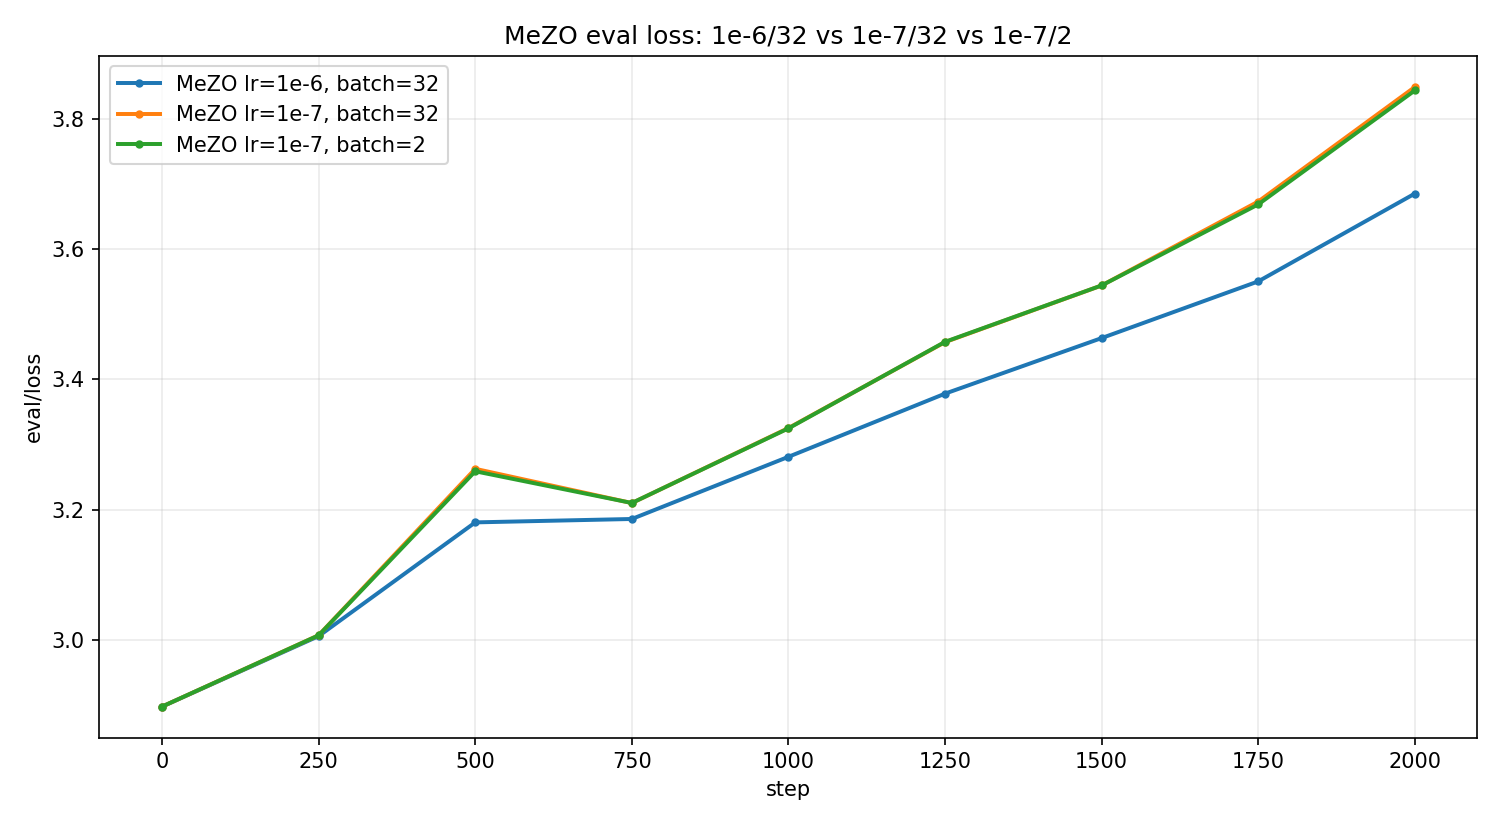
\includegraphics[width=1\textwidth]{images/eval_loss_mezo.png}
    \caption{Validation loss for MeZO with different learning rates and effective batch sizes. Step 0 corresponds to the evaluation of the base pretrained model before fine-tuning.}
    \label{fig:mezo-eval-loss}
\end{figure}

As shown in Figure~\ref{fig:mezo-eval-loss}, the validation loss increased steadily in all MeZO experiments. The effective batch size had almost no visible effect on this behavior, while reducing the learning rate did not stabilize training. This suggests that the observed degradation was not caused only by the magnitude of the final optimizer update.

\begin{table}[ht]
\centering
\begin{tabular}{ll}
\toprule
Parameter & Value \\
\midrule
Learning rate & 0 \\
Debug frequency & every step \\
Max steps & 10 \\
Train batch size & 1 \\
Eval batch size & 1 \\
Parameter dtype & bfloat16 \\
zo\_eps & $10^{-3}$ \\
\bottomrule
\end{tabular}
\caption{Configuration of the auxiliary debugging run.}
\end{table}

The debugging information was collected for three representative weight matrices from different parts of the model: \texttt{up\_proj} from the first MLP block, \texttt{q\_proj} from the first attention block, and \texttt{o\_proj} from the tenth attention block.

Since the learning rate was zero, no actual optimization update should have changed the model parameters. Ideally, after the full MeZO perturbation--restore cycle, the parameters should satisfy $\theta_{\mathrm{after}}=\theta_{\mathrm{before}}$. However, the debugging logs in Table~\ref{tab:mezo-lr-zero-restore} show that the inspected weight matrices were already modified after the perturbation--restore sequence. In this table, \texttt{restore\_max\_diff} is the maximum absolute difference between the original parameter values and the values after the perturbation was reverted, while \texttt{update\_max\_diff} is the final parameter difference after the optimizer update.

\begin{table}[ht]
\centering
\resizebox{\textwidth}{!}{%
\begin{tabular}{clcc}
\toprule
Step & Parameter & \texttt{restore\_max\_diff} & \texttt{update\_max\_diff} \\
\midrule
0 & \texttt{layers.0.mlp.up\_proj.weight}        & 0.001953 & 0.001953 \\
0 & \texttt{layers.0.self\_attn.q\_proj.weight}  & 0.007812 & 0.007812 \\
0 & \texttt{layers.10.self\_attn.o\_proj.weight} & 0.001953 & 0.001953 \\
\midrule
1 & \texttt{layers.0.mlp.up\_proj.weight}        & 0.000977 & 0.000977 \\
1 & \texttt{layers.0.self\_attn.q\_proj.weight}  & 0.003906 & 0.003906 \\
1 & \texttt{layers.10.self\_attn.o\_proj.weight} & 0.001953 & 0.001953 \\
\midrule
9 & \texttt{layers.0.mlp.up\_proj.weight}        & 0.001953 & 0.001953 \\
9 & \texttt{layers.0.self\_attn.q\_proj.weight}  & 0.007812 & 0.007812 \\
9 & \texttt{layers.10.self\_attn.o\_proj.weight} & 0.001953 & 0.001953 \\
\bottomrule
\end{tabular}%
}
\caption{Parameter restoration error in the auxiliary MeZO debugging run with zero learning rate. Even though no optimizer update should have been applied, the inspected \texttt{bfloat16} weight matrices were not restored exactly after zeroth-order perturbations.}
\label{tab:mezo-lr-zero-restore}
\end{table}

The key observation is that \texttt{restore\_max\_diff} and \texttt{update\_max\_diff} are identical. Since $\eta=0$, \texttt{update\_max\_diff} should also be zero. Therefore, the final parameter change was not caused by the optimizer update: it had already appeared during the perturbation--restore procedure. The observed restoration errors, $0.000977$, $0.001953$, $0.003906$, and $0.007812$, correspond to powers of two, $2^{-10}$, $2^{-9}$, $2^{-8}$, and $2^{-7}$. This is consistent with the coarse quantization of \texttt{bfloat16}. In other words, with $\epsilon=10^{-3}$, adding and then subtracting the same perturbation was not numerically reversible for these weights.

This numerical drift was also much larger than the intended MeZO update at the learning rates used in the main experiments. In the implementation, the scalar directional estimate is computed as

$$
\texttt{projected\_grad}
=
\frac{\texttt{loss\_diff}}{2 \cdot \texttt{zo\_eps}},
$$

and the parameter update has the form

$$
\Delta\theta
=
-\eta
\left(
\texttt{projected\_grad}\cdot z
+
\lambda\theta
\right),
$$

where $z$ is the sampled random direction and $\lambda$ is the weight decay coefficient.

Ignoring the weight decay term for an order-of-magnitude estimate,

$$
|\Delta\theta|
\sim
\eta \,
|\texttt{projected\_grad}|,
$$

since the components of $z$ are typically of order one.

In the zero-learning-rate debug run, the absolute values of \texttt{projected\_grad} had mean $9.71$, median $8.39$, and maximum $26.85$. Therefore, for $\eta=10^{-6}$, the typical intended update scale was approximately $8.4\cdot 10^{-6}$, with the largest observed estimate around $2.7\cdot 10^{-5}$. For $\eta=10^{-7}$, these values decrease to approximately $8.4\cdot 10^{-7}$ and $2.7\cdot 10^{-6}$. By contrast, the observed restoration errors ranged from $9.8\cdot 10^{-4}$ to $7.8\cdot 10^{-3}$. Thus, even at $\eta=10^{-6}$, the smallest observed restoration error was about $116$ times larger than the typical intended update and still about $36$ times larger than the largest observed update estimate. At $\eta=10^{-7}$, the restoration error exceeded the typical intended update by roughly three orders of magnitude.

This explains why decreasing the learning rate did not stabilize the validation loss. In this implementation, the model was gradually damaged even when the learning rate was zero, and for small nonzero learning rates the intended MeZO update was dominated by the numerical drift caused by non-reversible \texttt{bfloat16} perturbations.

\begin{figure}[ht]
    \centering
    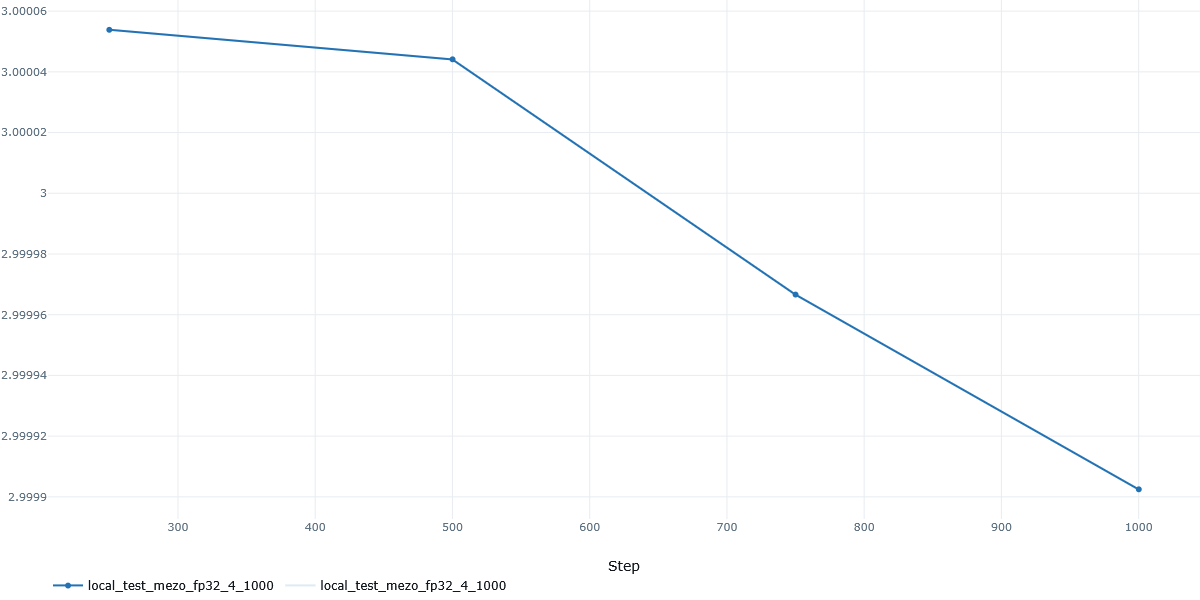
\includegraphics[width=1\textwidth]{images/eval_loss(7).png}
    \caption{Validation loss for MeZO with \texttt{float32}, $\eta=10^{-7}$, and batch size $2$.}
    \label{fig:mezo-fp32-loss}
\end{figure}

This interpretation is further supported by a short local control run with \texttt{float32}, $\eta=10^{-7}$, and \texttt{per\_device\_train\_batch\_size}=2, where the validation loss decreased instead of increasing (Figure~\ref{fig:mezo-fp32-loss}). Although this run was too short to compare final downstream quality, it indicates that the monotonic loss growth observed in the \texttt{bfloat16} runs was not an inherent consequence of MeZO itself, but was strongly tied to finite-precision perturbation errors.

\subsection{Model Quality}

\begin{table}[ht]
\centering
\resizebox{\textwidth}{!}{%
\begin{tabular}{llcccc}
\toprule
Optimizer & LR & Batch size & Train loss & Val loss 
& Avg harness score \\
\midrule
Base Qwen & - & - & - & - & 0.5365 \\
\midrule
AdamW & 5e-05 & 32 & 2.8840 & 2.8622 & 0.5407 \\
Muon & 5e-05 & 32 & 2.8838 & 2.8640 & 0.5424 \\
MeZO & 1e-06 & 32 & 3.3973 & 3.6856 & 0.5441 \\
MeZO & 1e-07 & 32 & 3.4656 & 3.8495 & 0.5449 \\
MeZO & 1e-07 & 2 & 3.3937 & 3.9049 & 0.5432 \\
\bottomrule
\end{tabular}%
}
\caption{Main quality metrics}
\label{tab:optimizer-comparison}
\end{table}

The metrics from \texttt{lm-evaluation-harness} produced interesting results despite the validation loss issue. On average, the scores remained close to the previous AdamW and Muon experiments and even showed a slight improvement, while individual task metrics varied noticeably.

The run with \texttt{per\_device\_train\_batch\_size}=2 is not included in the main optimizer comparison, since it was performed primarily to evaluate MeZO's memory efficiency and is not directly comparable to the other optimizers in terms of training setup. However, as shown in Table~\ref{tab:full-quality-metrics} and by the average score in Table~\ref{tab:optimizer-comparison}, this run produced results close to the batch size 32 run with the same learning rate.

\begin{table}[ht]
\centering
\begin{tabular}{llcccc}
\toprule
& & \multicolumn{2}{c}{ARC Challenge} & \multicolumn{2}{c}{ARC Easy} \\
\cmidrule(lr){3-4} \cmidrule(lr){5-6}
Optimizer & LR
& \texttt{acc} & \texttt{acc\_norm}
& \texttt{acc} & \texttt{acc\_norm} \\
\midrule
Base Qwen2.5-0.5B & -- & 0.2892 & 0.3200 & 0.6423 & 0.5816 \\
\midrule
AdamW    & $5 \cdot 10^{-5}$ & 0.2884 & 0.3225 & 0.6557 & 0.6330 \\
Muon     & $5 \cdot 10^{-5}$ & 0.2944 & 0.3268 & 0.6587 & 0.6296 \\
MeZO & $1 \cdot 10^{-6}$ & 0.2901 & 0.3131 & 0.6637 & 0.6237 \\
MeZO & $1 \cdot 10^{-7}$ & 0.2910 & 0.3140 & 0.6612 & 0.6233 \\
\bottomrule
\end{tabular}
\caption{ARC Easy and ARC Challenge results.}
\label{tab:arc-results}
\end{table}

ARC evaluates grade-school science question answering. ARC Easy contains simpler and more direct questions, ARC Challenge contains more difficult questions that are typically answered incorrectly by retrieval-based or simpler baseline methods. 

For the ARC tasks, MeZO also achieved relatively strong results, similarly to AdamW and Muon. However, the two ARC metrics show different behavior. In terms of raw accuracy, MeZO remained stable and achieved results comparable to or higher than those of AdamW and Muon. In contrast, the length-normalized accuracy was lower for MeZO, and on ARC Challenge it even decreased relative to the base model.

\begin{table}[ht]
\centering
\begin{tabular}{llcccc}
\toprule
& & \multicolumn{2}{c}{HellaSwag} & \multicolumn{2}{c}{PIQA} \\
\cmidrule(lr){3-4} \cmidrule(lr){5-6}
Optimizer & LR
& \texttt{acc} & \texttt{acc\_norm}
& \texttt{acc} & \texttt{acc\_norm} \\
\midrule
Base Qwen2.5-0.5B & -- & 0.4059 & 0.5210 & 0.7046 & 0.6970 \\
\midrule
AdamW    & $5 \cdot 10^{-5}$ & 0.3984 & 0.5025 & 0.6959 & 0.6921 \\
Muon     & $5 \cdot 10^{-5}$ & 0.3989 & 0.5032 & 0.6970 & 0.6942 \\
MeZO & $1 \cdot 10^{-6}$ & 0.3968 & 0.5130 & 0.6953 & 0.6991 \\
MeZO & $1 \cdot 10^{-7}$ & 0.3973 & 0.5133 & 0.6926 & 0.6991 \\
\bottomrule
\end{tabular}
\caption{HellaSwag and PIQA results.}
\label{tab:hellaswag-piqa-results}
\end{table}

HellaSwag and PIQA evaluate commonsense reasoning in physical and everyday scenarios. PIQA focuses more directly on physical interaction and affordance understanding, while HellaSwag tests the model's ability to select the most plausible continuation of a given situation.

On these physically grounded tasks, MeZO mostly decreased the model's performance, similarly to AdamW and Muon in the main part of the study. It is also noticeable that, for these tasks, raw accuracy decreased more strongly than length-normalized accuracy. In some cases, such as PIQA, \texttt{acc\_norm} remained close to the base model result, while \texttt{acc} showed a clearer degradation.

\begin{table}[ht]
\centering
\begin{tabular}{llc}
\toprule
Optimizer & LR & WinoGrande \\
\midrule
Base Qwen2.5-0.5B & -- & 0.5627 \\
\midrule
AdamW    & $5 \cdot 10^{-5}$ & 0.5533 \\
Muon     & $5 \cdot 10^{-5}$ & 0.5580 \\
MeZO & $1 \cdot 10^{-6}$ & 0.5714 \\
MeZO & $1 \cdot 10^{-7}$ & 0.5746 \\
\bottomrule
\end{tabular}
\caption{WinoGrande results.}
\label{tab:winogrande-results}
\end{table}

WinoGrande evaluates commonsense reasoning through pronoun and reference resolution. Each example contains a sentence with a missing entity, and the model must choose which of two candidates makes the sentence coherent.

This task produced the most nontrivial result among the downstream evaluations. Unlike AdamW and Muon, which slightly decreased the model's WinoGrande score in the main experiments, MeZO showed a small improvement. Although the gain was not large, WinoGrande is the only task where MeZO clearly differs from AdamW and Muon.

\subsection{Analysis}
Overall, the downstream metrics suggest a mixed and unstable picture. MeZO performed best on tasks where the answer is selected from short candidates or where the decision depends mainly on local ranking. This is visible in WinoGrande, formulated as a binary choice between two short candidates, and in ARC, where the improvement appeared mainly in raw \texttt{acc} but not in \texttt{acc\_norm}.

This difference between \texttt{acc} and \texttt{acc\_norm} is important. Raw accuracy selects the answer with the highest total log-likelihood, whereas normalized accuracy uses average log-likelihood per token. Therefore, an increase in \texttt{acc} together with a decrease in \texttt{acc\_norm} suggests that the improvement is sensitive to the scoring rule. In the ARC tasks, this makes the gain less robust: it may reflect changes in answer length bias, answer priors, or the ranking of borderline examples rather than a stable improvement in task understanding.

A similar scoring-dependent behavior appears on physically grounded tasks such as HellaSwag and PIQA. On these benchmarks, MeZO, similarly to the other optimizers, mostly decreased the base model performance. The degradation was more pronounced in raw \texttt{acc}, while \texttt{acc\_norm} changed less. This supports the interpretation that MeZO changed the relative ranking of answer choices rather than uniformly improving or degrading all downstream abilities.

Together with the steadily increasing train and validation loss, these results suggest that MeZO in this configuration did not train the model in a stable way. Instead, it likely introduced a noisy shift in the model's probability distribution. This shift degraded general language-modeling quality, but could still improve some multiple-choice metrics by changing length bias, answer priors, or the ordering of close candidate answers.

Thus, the observed downstream improvements should be interpreted cautiously. In this configuration, MeZO did not consistently improve model quality; rather, it changed the model's ranking behavior in a way that helped some metrics while harming others.

\subsection{Computational Resources}

\begin{table}[ht]
\centering
\resizebox{\textwidth}{!}{%
\begin{tabular}{llcccc}
\toprule
Optimizer & LR & Batch size & Training time (s) & Max memory (MB) & Avg harness score \\
\midrule
AdamW & $5 \cdot 10^{-5}$ & 32 & 5156.04 & 8803.88 & 0.5407 \\
Muon & $5 \cdot 10^{-5}$ & 32 & 5402.74 & 8122.34 & 0.5424 \\
MeZO & $1 \cdot 10^{-6}$ & 32 & 1878.52 & 48496.29 & 0.5441 \\
MeZO & $1 \cdot 10^{-7}$ & 32 & 1878.92 & 48496.29 & 0.5449 \\
MeZO & $1 \cdot 10^{-7}$ & 2 & 1092.60 & 3932.57 & 0.5432 \\
\bottomrule
\end{tabular}%
}
\caption{Training time, maximum memory usage, and final quality.}
\label{tab:resource-efficiency}
\end{table}

The resource measurements show that MeZO was faster than both backpropagation-based optimizers. The batch size $32$ MeZO runs took about $1879$ seconds, compared with $5156$ seconds for AdamW and $5403$ seconds for Muon. The smaller batch size $2$ MeZO run was even faster, taking $1093$ seconds.

Memory usage depended strongly on the microbatch size. With batch size $2$, MeZO used only $3932.57$ MB, compared with $8803.88$ MB for AdamW and $8122.34$ MB for Muon. This confirms the practical memory advantage of avoiding backpropagation under comparable microbatch conditions.

However, matching the effective batch size required MeZO to use batch size $32$ in a single forward pass, since gradient accumulation was not used. This increased peak memory to $48496.29$ MB. Although this is still consistent with MeZO's theoretical memory savings relative to a backpropagation-based optimizer at the same microbatch size, it removed the practical memory advantage in this setup.

The larger MeZO batch also did not substantially improve final quality: with the same learning rate, batch size $2$ achieved an average harness score of $0.5432$, while batch size $32$ achieved $0.5449$. Thus, the additional memory cost was not justified by a comparable gain in downstream performance.

\section{Conclusion}
The MeZO results are quite difficult to interpret. Despite the chaotic behavior of training loss and the steady degradation of validation loss, some \texttt{lm-evaluation-harness} metrics still show improvements that are close to, and in some cases even slightly exceed, the results of the backpropagation-based optimizers AdamW and Muon, although these differences remain close to the range of random fluctuations.

The main reason for the loss degradation is related not so much to MeZO itself as to the chosen numerical configuration. A debugging run with \texttt{learning\_rate}=0 showed that, with \texttt{bfloat16} and \texttt{zo\_eps}=$10^{-3}$, the model weights were already changing during the perturbation--restore procedure. In other words, the model was being damaged even without an optimizer update. At small learning rates, the useful MeZO update was substantially smaller than this restoration error, so decreasing the learning rate did not stabilize training.

The experimental setup also differed from the original MeZO paper. In the paper, MeZO was mainly applied to task-specific supervised fine-tuning, where the data are given as input-output examples and the training objective is directly connected to the target downstream task. In this work, a general language-modeling objective on \texttt{openwebtext-100k} was used. Such a setup provides only an indirect signal for improving ARC, PIQA, HellaSwag, and WinoGrande. Therefore, it is less favorable for a noisy zeroth-order method.

Thus, as analyzed above, it can be assumed that the result was mostly caused by a noisy shift in the model's probability distribution. However, the fact that the metric results are close to those of AdamW and Muon may cast some doubt on this conclusion. Based on this set of training runs, the results have to be considered ambiguous and requiring further experiments.

The final conclusion for this experiment is as follows: in the current configuration, MeZO was efficient in terms of training time and potentially efficient in terms of memory at a small microbatch size, but stable model improvement remains questionable. Its downstream results are explained primarily by a change in ranking behavior on multiple-choice tasks rather than by a stable improvement in language modeling.
\appendix

\section{Appendix}

\clearpage
\begin{sidewaystable}[p]
\centering
\small
\resizebox{\textheight}{!}{%
\begin{tabular}{lllccccccccccc}
\toprule
Optimizer & LR & Batch size & Train loss & Val loss 
& ARC-C & ARC-C norm 
& ARC-E & ARC-E norm 
& HellaSwag & HellaSwag norm 
& PIQA & PIQA norm 
& WinoGrande \\
\midrule
base\_qwen & - & - & - & - & 0.2892 & 0.3200 & 0.6423 & 0.5816 & 0.4059 & 0.5210 & 0.7046 & 0.6970 & 0.5627 \\
adamw & 5e-05 & 32 & 2.8840 & 2.8622 & 0.2884 & 0.3225 & 0.6557 & 0.6330 & 0.3984 & 0.5025 & 0.6959 & 0.6921 & 0.5533 \\
muon & 5e-05 & 32 & 2.8838 & 2.8640 & 0.2944 & 0.3268 & 0.6587 & 0.6296 & 0.3989 & 0.5032 & 0.6970 & 0.6942 & 0.5580 \\
\midrule
mezo & 1e-06 & 32 & 3.3973 & 3.6856 & 0.2901 & 0.3131 & 0.6637 & 0.6237 & 0.3968 & 0.5130 & 0.6953 & 0.6991 & 0.5714 \\
mezo & 1e-07 & 32 & 3.4656 & 3.8495 & 0.2910 & 0.3140 & 0.6612 & 0.6233 & 0.3973 & 0.5133 & 0.6926 & 0.6991 & 0.5746 \\
mezo & 1e-07 & 2 & 3.3937 & 3.9049 & 0.3063 & 0.3302 & 0.6494 & 0.6183 & 0.3986 & 0.5157 & 0.6937 & 0.6888 & 0.5675 \\
\bottomrule
\end{tabular}%
}
\caption{Full downstream evaluation results.}
\label{tab:full-quality-metrics}
\end{sidewaystable}
\clearpage

\end{document}